\documentclass[10pt,a4paper]{article}
\usepackage[utf8]{inputenc}
\usepackage[italian]{babel}
\usepackage{amsmath}
\usepackage{amsfonts}
\usepackage{amssymb}
\usepackage{graphicx}
\usepackage[left=2cm,right=2cm,top=2cm,bottom=2cm]{geometry}
\newcommand{\rem}[1]{[\emph{#1}]}
\newcommand{\exn}{\phantom{xxx}}

\author{Gruppo xx.y \\ Mario Rossi, Anna Bianchi \rem{non dimenticate i nomi}}
\title{Es03: Amplificatore ad emettitore comune con BJT}
\begin{document}
\date{23 ottobre 2150 \rem{idem per la data}}
\maketitle

\section*{Schema del circuito e misura dei componenti circuitali}
Il circuito che implementa un amplificatore ad emettitore comune con BJT \'e mostrato in figura~\ref{fig:circuit}.
\begin{figure}[htp]
\begin{center}
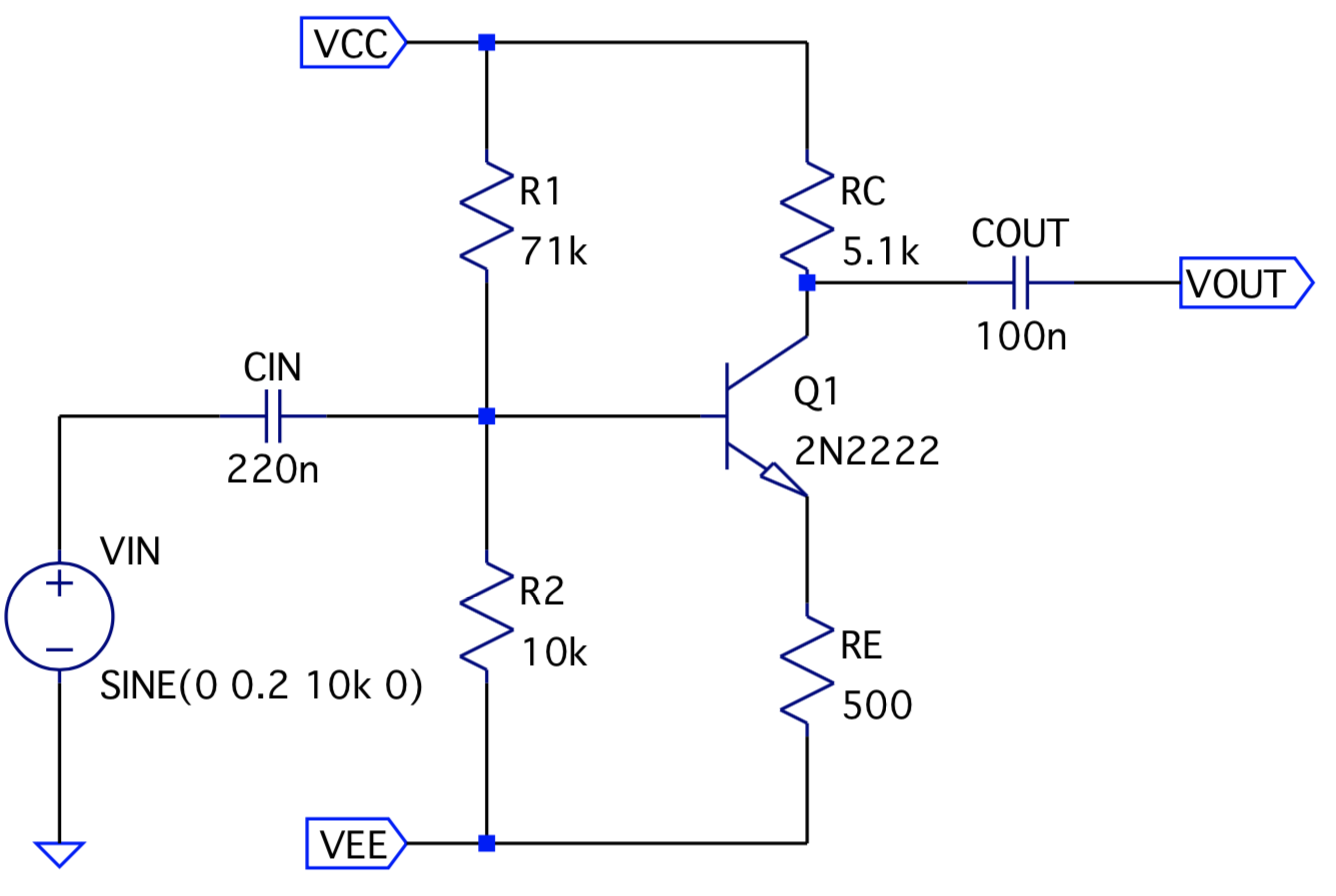
\includegraphics[scale=0.5]{AmplBJT-B.png}
\caption{Schema circuitale amplificatore ad emettitore comune con BJT.}
\label{fig:circuit}
\end{center}
\end{figure}
Il valore dei componenti utilizzati sono (per la nomenclatura riferirsi allo schema di figura~\ref{fig:circuit}):
\[
\begin{array}{rcl}
R_1 &=& (\ldots \pm \ldots) \mathrm{k}\Omega\\
R_2 &=& (\ldots \pm \ldots) \mathrm{k}\Omega\\
R_C &=& (\ldots \pm \ldots) \mathrm{k}\Omega\\
R_E &=& (\ldots \pm \ldots) \mathrm{k}\Omega\\
C_{in} &=& (\ldots \pm \ldots) \mathrm{nF}\\
C_{out} &=& (\ldots \pm \ldots) \mathrm{nF}
\end{array}
\]


\setcounter{section}{0}
\section{Verifica del punto di lavoro}

\subsection*{a) Polarizzazione del BJT, misura delle componenti quiescenti}
Con $V_{IN}$ sconnesso ed utilizzando il voltmetro digitale rispettivamente con fondo-scala $\ldots$ per la misura di $V_{BE}$, $\ldots$ per quella di $V_{CE}$ e $\ldots$ per la d.d.p. ai capi di $R_C$, abbiamo ottenuto i valori riportati in tabella per la misura delle componenti quiescenti di quelle grandezze, confrontati con quelli attesi.
\begin{table}[h]
\centering
\begin{tabular}{|c|l|l|}
\hline
\hline 
& misurato & atteso\\
\hline
$V_{BE}^Q$ & $ (\dots \pm \ldots) \,\mathrm{V}$  & $ (\dots \pm \ldots) \,\mathrm{V}$  \\
\hline 
$V_{CE}^Q$ & $ (\dots \pm \ldots) \,\mathrm{V}$  & $ (\dots \pm \ldots) \,\mathrm{V}$  \\
\hline
$I_C^Q$ & $ (\dots \pm \ldots) \,\mathrm{mA}$  & $ (\dots \pm \ldots) \,\mathrm{mA}$  \\
\hline 
\hline
\end{tabular} 
\caption{Valori misurati ed attesi per le componenti quiescenti al punto di lavoro del BJT.}
\label{tab:quiescente}
\end{table}
Per il calcolo delle incertezze sulle misure di tensione si \`e considerato....
%
\subsection*{b) Stima di $h_{FE}$, verifica della rigidit\`a del partitore}
Abbiamo misurato i seguenti valori per le d.d.p. ai capi di $R_1$ ed $R_2$:
\[
V_1^Q = (\dots \pm \ldots) \,\mathrm{V}, \;V_2^Q = (\dots \pm \ldots) \,\mathrm{V}
\]
da cui, dividendo per le rispettive resistenze e calcolando la differenza, risulta per la corrente quiescente di base:
\[ 
I_1^Q = V_1^Q/R_1 = (\dots \pm \ldots) \,\mu\mathrm{A},\;I_2^Q = V_2^Q/R_2 = (\dots \pm \ldots) \,\mu\mathrm{A}
\]
\[
\Rightarrow I_B^Q =  I_1^Q - I_2^Q = (\dots \pm \ldots) \,\mu\mathrm{A}
\]
Dal rapporto della componente quiescente della corrente di collettore e di quella di base otteniamo infine una stima del 
guadagno in corrente del transistor di $h_{FE} = \ldots \pm \ldots$.\\
\vspace{0.5cm}
\framebox(400,30){Inserire un commento sulla rigidit\`a del partitore basato sul confronto delle correnti.}

\section{Risposta a centro-banda}
\subsection*{a) Sfasamento}
Inviando all'~ingresso dell'~amplificatore un segnale sinusoidale di frequenza $10$~kHz ed ampiezza $200$~mV, osserviamo in 
ingresso/uscita le forme d'~onda riportate in figura \ref{fig:osci} registrate su Ch1/Ch2 dell'~oscilloscopio:
\begin{figure}[htp]
\centering
%\includegraphics[scale=0.4]{part1.pdf}
\framebox(400,50){Inserire l'~immagine dell'~oscilloscopio dopo opportuna regolazione dei fondo-scala.}
\caption{Segnali di ingresso/uscita per l'amplificatore a centro-banda.}
\label{fig:osci}
\end{figure}
\vspace{0.5cm}
\framebox(400,30){Inserire un commento su quanto osservato ed una misura dello sfasamento tra $V_{in}$ e $V_{out}$.}

\subsection*{b) Misura del guadagno}
Fissata la frequenza di $V_{IN}$ al valore precedente, ne abbiamo variato l'~ampiezza in un intervallo di linearit\`a dell'~uscita. I 
valori misurati per le ampiezze sono riportati in tabella \ref{tab:lin}. \fbox{Spiegare come sono stati ottenuti}  

\begin{table}[h]
\caption{Ampiezza segnali di ingresso/uscita in zona lineare dell'~amplficatore}
\label{tab:lin}
\begin{center}
\begin{tabular}{|c|c|}
\hline 
\hline 
$V_{in}$ (mV)  & $V_{out}$ (V)\\
\hline 
$\ldots \pm \ldots$ & $\ldots \pm \ldots$  \\
\hline 
$\ldots \pm \ldots$ & $\ldots \pm \ldots$  \\
\hline 
$\ldots \pm \ldots$ & $\ldots \pm \ldots$  \\
\hline 
$\ldots \pm \ldots$ & $\ldots \pm \ldots$  \\
\hline 
$\ldots \pm \ldots$ & $\ldots \pm \ldots$  \\
\hline 
$\ldots \pm \ldots$ & $\ldots \pm \ldots$  \\
\hline 
$\ldots \pm \ldots$ & $\ldots \pm \ldots$  \\
\hline 
\hline 
\end{tabular} 
\end{center}
\end{table}

Mediante interpolazione lineare dei punti misurati otteniamo \fbox{spiegare con quale funzione avete interpolato i dati} il grafico
mostrato in figura \ref{fig:fit} ed i seguenti parametri del fit:
\[
\begin{array}{rcl}
A_v &=& (\ldots \pm \ldots) \\
\chi^2/ndof &=&\ldots/\ldots
\end{array}
\]
\begin{figure}[htp]
\begin{center}
%\includegraphics[scale=0.4]{part1.pdf}
\framebox(400,30){Inserire sopra il plot di $V_{OUT}$ vs $V_{IN}$ con la retta di best-fit}
\framebox(400,30){Inserire sotto il grafico dei residui normalizzati}
\caption{$V_{OUT}$ in funzione di $V_{IN}$ nella zona di linearit\`a dell'amplificatore, con sovrapposta funzione di best-fit.}
\label{fig:fit}
\end{center}
\end{figure}


\subsection*{c) Limiti di linearit\`a}
L'~uscita si mantiene lineare finch\'e l'~ampiezza dell'~ingresso non raggiunge un valore $V_{in} = (\ldots \pm \ldots) \,\mathrm{mV}$, in corrispondenza del quale si osserva il {\it clipping} della concavit\`a \dots di $V_{out}$, come appare nel plot a sinistra di figura \ref{fig:clipping}.
\framebox(500,50){Discutere come in corrispondenza di quel limite il BJT esca dalla zona di linearit\`a.}
%
\begin{figure}[htp]
\begin{center}
\framebox(200,200){Clipping di $V_{out}$ sulla sua semi-onda \dots}
\framebox(200,200){Clipping di $V_{out}$ su entrambe le semi-onde}
%\includegraphics[0.45\textwidth]{}
%\includegraphics[0.45\textwidth]{}
\end{center}
\caption{Clipping di $V_{out}$ per ampiezza $V_{in} = \ldots$ (sinistra) e $V_{in} = \ldots$ (destra). }
\label{fig:clipping}
\end{figure}
%

\subsection*{d) Simmetria del clipping e punto di lavoro}
Aumentando ulteriormente l'~ampiezza dell'˜ingresso oltre $V_{in} = (\ldots \pm \ldots) \,\mathrm{mV}$ il segnale di uscita satura 
anche sulla semi-onda \dots, come mostrato a destra in figura \ref{fig:clipping}.\\
\fbox{\begin{minipage}{\textwidth}
Discutere l'~asimmetria del clipping in 
termini dell'~asimmetria del punto di lavoro sulla retta di carico e mettere in relazione ciascuno stato con la polarizzazione del 
BJT (per una migliore comprensione potrebbe essere utile visualizzare $V_B$ e $V_C$, quest'~ultimo a monte di $C_{out}$.)
\end{minipage}}

%
\section{Risposta in frequenza}
\subsection*{a) Plot di Bode}
Mediante l'~utilizzo del Network Analyzer abbiamo ottenuto i plot di Bode in ampiezza e fase mostrati in figura \ref{fig:bode}.\\
\fbox{\begin{minipage}{\textwidth}
Ottimizzate le scale per una migliore visualizzazione (ad es. conviene per ovvi motivi fissare a 180 gradi l'offset della fase). Fate 
in modo che sullo screenshot siano leggibili le impostazioni; in caso contrario riportatele esplicitamente nel testo.
\end{minipage}}
%
\begin{figure}[htp]
\begin{center}
%\includegraphics[scale=0.4]{part1.pdf}
\framebox(400,30){Inserire lo screenshot con i plot di Bode}
\caption{Plot di Bode in ampiezza (sopra) e fase (sotto) per l'~amplificatore.}
\label{fig:bode}
\end{center}
\end{figure}

\subsection*{b) Frequenze di taglio}
Dal plot precedente abbiamo stimato i seguenti valori per le frequenze di taglio dell'~amplificatore:
\[
\left\{
\begin{array}{lcl}
\mbox{frequenza di taglio inferiore} &=& f_{HP} = (\exn \pm \exn)\,\mbox{Hz}\\
\mbox{frequenza di taglio superiore} &=& f_{LP} = (\exn \pm \exn)\,\mbox{kHz}
\end{array}
\right.
\]
\fbox{\begin{minipage}{12cm}
Spiegate il metodo utilizzato ed il criterio seguito nella stima delle incertezze.
\end{minipage}}
%
\subsection*{c) Frequenza di taglio inferiore, confronto con il valore atteso}
La frequenza di taglio inferiore discende dal filtro passa-alto posto sullo stadio di ingresso dell'~amplificatore, il cui valore atteso \`e 
\[
\bar{f}_H = \mbox{scrivere formula in termini dei componenti circuitali} = (\exn \pm \exn) \, \mathrm{Hz}
\]
\fbox{\begin{minipage}{\textwidth}
Discutere il confronto (accordo o ragioni di eventuali discrepanze) tra $f_H$ ed $\bar{f}_H$. 
\end{minipage}}
\subsection*{d) Andamento ad alte frequenze}
\fbox{\begin{minipage}{\textwidth}
Discutere qualitativamente l'~andamento del guadagno intorno alla frequenza di taglio superiore sulla base del modello del BJT ad alta frequenza e grossolanamente (ovvero a livello di ordini di grandezza), il suo accordo con quanto atteso. 
\end{minipage}}.
\section*{Conclusioni e commenti finali}
\framebox(400,30){Inserire eventuali commenti e conclusioni finali}

\section*{Dichiarazione}
I firmatari di questa relazione dichiarano che il contenuto della relazione \`e originale, con misure effettuate dai membri del gruppo, e che tutti i firmatari hanno contribuito alla elaborazione della relazione stessa.

\end{document}